% Number 450
% BFPM Springs
% Spring holding object at rest - a bit tricky with length
% MIT

% Watermark
\AddToShipoutPicture*{\BackgroundPic}

\addtocounter {ProbNum} {1}

%\begin{floatingfigure}[r]{.35\textwidth}
%\includegraphics[scale=.5]{/Users/jgates/desktop/latex/pics/staticeq1.png}
%\end{floatingfigure}
 
{\bf \Large{\arabic{ProbNum}}} An 8.4 kg mass is suspended from a spring with spring constant ${450~\tfrac{N}{m}}$.  This causes the spring to have a total length of 0.390 m. 

\bigskip
Find the new total length of the spring when a 13.4 kg mass is suspended from it.

%\begin{center}
%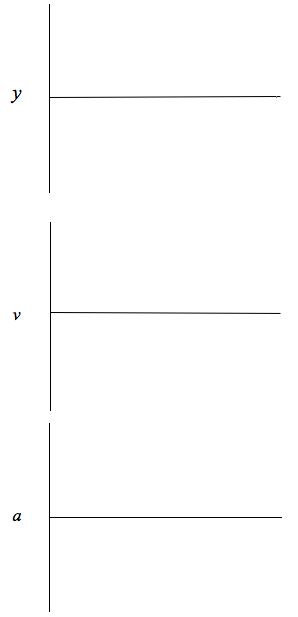
\includegraphics[scale=.85]{/Users/jgates/desktop/latex/pics/blankyvagraphstack.png}
%\end{center}


\vfill
\newpage